\documentclass[11pt,letterpaper]{article}
\usepackage[margin=.85in]{geometry}
\usepackage{amsmath,amssymb,booktabs,tabularx,array,xcolor,hyperref,fancyhdr,tikz,enumitem}
\usetikzlibrary{positioning,arrows.meta}
\definecolor{navy}{HTML}{15334D}
\definecolor{teal}{HTML}{087F83}
\hypersetup{colorlinks=true,linkcolor=teal,urlcolor=teal}
\pagestyle{fancy}\fancyhf{}\lhead{\small\color{navy} BAYESIAN HALLUCINATION REGIME LAB}\rhead{\small Research blueprint}\cfoot{\thepage}
\setlength{\headheight}{15pt}
\setlength{\emergencystretch}{2em}
\setlength{\parindent}{0pt}\setlength{\parskip}{6pt}
\newcommand{\Hstate}{\mathrm{H}}
\newcommand{\E}{\mathbb E}
\newcommand{\Var}{\operatorname{Var}}
\newcommand{\Prob}{\mathbb P}
\newcommand{\R}{\mathbb R}
\newcommand{\sectionpage}[1]{\clearpage\section{#1}}
\begin{document}
\begin{titlepage}
\color{navy}
\vspace*{1.2cm}
{\Large\textbf{RESEARCH PROTOCOL / IMPLEMENTATION BLUEPRINT}}\\[1cm]
{\Huge\bfseries Bayesian Hallucination\\ Regime Lab}\\[.5cm]
{\LARGE Detection, forecasting, factor attribution and intervention with covariate-dependent hidden Markov models}\\[1cm]
\rule{\linewidth}{2pt}
\vspace{.6cm}

{\large Prepared for Nihar Narsana\\ MS Data Science --- Bayesian Inference and Modelling\\ University of Arizona}\\[.7cm]
\textbf{Status:} Proposed research and software specification; implementation awaits approval.\\
\textbf{Version:} 1.0 --- November 2026

\vfill
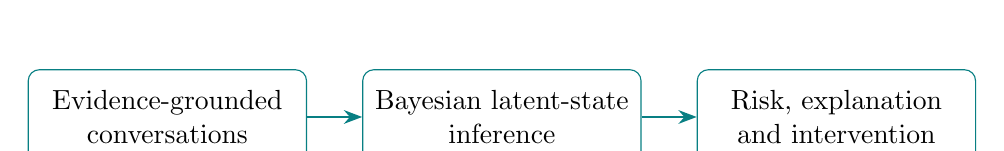
\begin{tikzpicture}[node distance=7mm, every node/.style={draw=teal, rounded corners, align=center, minimum height=12mm, text width=3.3cm}, >=Stealth]
\node (a) {Evidence-grounded\\ conversations};
\node[right=of a] (b) {Bayesian latent-state\\ inference};
\node[right=of b] (c) {Risk, explanation\\ and intervention};
\draw[->,thick,teal] (a)--(b);\draw[->,thick,teal] (b)--(c);
\end{tikzpicture}

\vspace{.5cm}
\textbf{Scientific principle:} Do not assume that hallucinations form persistent regimes. Test that hypothesis, quantify uncertainty, and distinguish statistical association from controlled causal effects.
\end{titlepage}
\tableofcontents
\sectionpage{Executive research design}
\textbf{Problem.} A language model may give an unsupported answer and then elaborate on its own earlier error. Standard independent classifiers ignore sequence information. A hidden Markov model (HMM) carries forward uncertainty over underlying regimes. A covariate-dependent Bayesian HMM additionally estimates how observed conditions change transition probabilities. Neither model directly observes the internal reason a model is wrong.

\textbf{Primary question.} Under identical emissions and identical evidence, does causal sequence filtering improve detection of the first unsupported answer, compared with a static mixture detector?

\textbf{Secondary questions.} Can the posterior predict a future error before the next answer? Which measurable pre-answer conditions are associated with transitions to hallucination? Does correcting a previous error or restoring evidence reduce later unsupported answers under randomized interventions?

\textbf{Scope.} Closed-evidence fictional structured QA; six turns per dossier; one quantized local Qwen checkpoint; 500 independent dossiers after a separate five-dossier pilot. Controlled fictional facts permit independent grading without an LLM judge. Study turn-level detection, not token-level interruption or open-world truth. A halt before the next question cannot undo the already emitted claim.


\begin{tabularx}{\linewidth}{p{.25\linewidth}X}
\toprule Aim & Falsifiable outcome \\ \midrule
A1: Temporal value & Paired held-out onset AUROC difference (filter minus matched static) with dossier bootstrap interval. \\
A2: Bayesian uncertainty & Posterior predictive calibrated risk; credible intervals; convergence and coverage under simulation. \\
A3: Factor gaps & Posterior contrasts for evidence, ambiguity, context noise and other pre-answer covariates. No claimed cause from coefficients alone. \\
A4: Intervention & Randomized paired difference in reference-graded next-turn errors, with uncertainty. \\
A5: Research system & Reproducible pipeline, exact numerical oracles, figures, dashboard and independently auditable results. \\ \bottomrule
\end{tabularx}

\textbf{Evidence status.} The supplied research report describes a starter synthetic study: 180 ten-turn sequences; 36 held-out sequences; 19 onsets / 282 at-risk turns; AUROC 0.843 HMM, 0.852 matched static and 0.674 single feature. HMM minus static was -0.009 (paired 95\% interval [-0.040, 0.020]). These are reported historical simulation results, not newly reproduced results or measurements of Qwen. The starter archive could not be downloaded because of DNS failure. Inspect and reuse it when accessible; otherwise implement compatible contracts from scratch.

\sectionpage{Research positioning and hypotheses}
Use the supplied \emph{Hallucination Onset Research Report} and \emph{Implementation Brief} as the predecessor specifications. The literature already includes sequential monitoring, so the novelty is not inventing an HMM or claiming the first hallucination monitor. The defensible contribution is a controlled matched-emission comparison plus uncertainty-aware transition attribution and paired experiments.


\begin{tabularx}{\linewidth}{p{.32\linewidth}X}
\toprule Prior direction & Implication for this project \\ \midrule
Zhang et al., hallucination snowballing & Retain actual preceding answers; compare corrected and original prefixes separately. \\
Wu et al., synchronous faithfulness monitoring & Compare shared features rather than attributing all gains to history. \\
RAGTruth & Independent annotations and grounding taxonomy; independent responses do not automatically make sequences. \\
SelfCheckGPT; semantic entropy & Optional expensive baselines; token entropy is not semantic entropy. \\
Lookback Lens & Attention-based context reliance is an optional feature study, not a causal explanation. \\
Rabiner; Bayesian HMM methodology & Exact recursions, latent-state non-identifiability, posterior inference. \\ \bottomrule
\end{tabularx}

\textbf{Preregistered hypotheses.}
\begin{enumerate}[label=H\arabic*.]
\item Sequential filtering changes first-onset discrimination relative to static scoring. Report either direction and paired interval.
\item Error persistence exceeds that expected from independent turns after accounting for dossier difficulty and turn type. Compare empirical transitions, posterior predictive checks and an independent-state model.
\item Pre-answer evidence availability and ambiguity change transition risk; signs are not imposed by the prior.
\item Parameter-integrated forecasts are at least as well calibrated as plug-in HMM forecasts in held-out data; test with Brier score and log score.
\item Randomly correcting a prior wrong answer changes next-turn error frequency relative to a matched original-prefix branch.
\end{enumerate}
Predeclare one primary estimand; treat the remaining analyses as secondary or exploratory. Avoid choosing a favorable endpoint after looking at test results. Report negative and inconclusive outcomes.

\sectionpage{Data design and independent truth}
\textbf{Collection contract.} Four fictional entities, four fields per entity, unique codes with controlled shared-code distractors, six questions including lookup, reference to prior entity, ambiguity and missing field. Store the visible dossier, complete conversation, question type, entity and authoritative answer in separate raw and grading artifacts. Generate questions from a seeded template, not model outputs. Maintain previous assistant responses in uninterrupted conversations.


\begin{tabularx}{\linewidth}{p{.17\linewidth}X}
\toprule Reference label & Operational definition \\ \midrule
G (grounded) & Correct supported code or warranted UNKNOWN when evidence is absent. \\
U (uncertain) & Explicit abstention when an answer is supported. \\
H (unsupported) & Wrong entity-code, invented code or unsupported assertion, even when confident. \\
Pending & Ambiguous or malformed prose, empty output or disputed label. Review blind to scores; retain reason and original record. \\ \bottomrule
\end{tabularx}

\textbf{Splits.} Assign 300/100/100 dossiers to train/validation/test before fitting, grouping related variants and intervention branches. Pilot IDs start at 10000; main IDs 0--499; guarded examples start at 20000. Separate pilot, synthetic, real uninterrupted and guarded data by manifest. Never split individual turns across folds.

\textbf{Primary observations} $x_{nt}\in\R^3$: selected-token mean log probability $\ell$, mean entropy $e$, maximum lexical cosine $s$. For generated non-stop tokens $y_k$ with full predictive distribution $p_k(v)$,
\[
\ell=\frac1L\sum_k\log p_k(y_k),\qquad
e=-\frac1L\sum_k\sum_v p_k(v)\log p_k(v).
\]
For word-count vectors $u(a)$ of answer and $u(r)$ of source row, $s=\max_r u(a)^\top u(r)/(\|u(a)\|\|u(r)\|)$. Set cosine to zero for empty vectors; mark missing token statistics and empty generations ineligible under the locked policy. Do not silently impute absent entropy. Record whether logits precede sampling transformations. Use only visible source rows, not gold row identity.

\textbf{Provenance.} Record model revision, checkpoint, package versions, seeds, sampler, token cap (32), temperature (0.7), prompt hash, timing, feature schema, review status and eligibility. Use atomic JSON writes and resume only compatible complete records. Primary labels never enter inference features. Source metadata used in explanatory models must be legitimately available at prediction time.

\sectionpage{Covariates and the meaning of a gap}
Separate predictors by availability, and distinguish a fact-checking oracle from a risk detector.

\begin{tabularx}{\linewidth}{p{.24\linewidth}p{.19\linewidth}X}
\toprule Factor & Timing & Operationalization \\ \midrule
Evidence availability & Before answer & Visible field coverage or experimentally assigned missingness; do not expose expected code. \\
Referential ambiguity & Before answer & Number of candidate entities or template ambiguity indicator. \\
Distractor burden & Before answer & Shared-code count or irrelevant rows assigned by design. \\
Context length & Before answer & Token count in visible prompt. Control turn number separately. \\
Prior model risk & Before answer & Previous causal filtered risk, only in separately evaluated model; avoid circular reuse of state probabilities. \\
Temperature & Before answer & Randomized sampling setting in a secondary study, constant in primary run. \\
Entropy, log probability & After answer & Emission observations; unavailable for next-turn forecast until answer is generated. \\
Lexical grounding & After answer & Similarity to evidence; can be high for a wrong entity. \\
Reference error history & Audit only & Actual earlier labels; never a live input unless a verified correction is explicitly available. \\ \bottomrule
\end{tabularx}

\textbf{Three explanation types.} (1) Observation attribution: how current features alter the posterior, e.g., use leave-one-feature-out marginal emissions and show the risk difference. (2) Transition attribution: how pre-answer conditions alter likelihood of entering or staying in H. (3) Intervention effects: how changing conditions in randomized trials affects independently graded outcomes. None proves a mechanistic reason inside the neural model.

\textbf{Gap audit.} For each high-risk or false-negative turn display evidence rows, resolved question for human audit, actual answer, independent label, current feature values, posterior state risk, transition constraints and missing-information indicators. Explicitly identify high-confidence wrong-entity cases. Label every explanation as model-based association, not a fact about cognition.

\sectionpage{Probability foundations and graphical model}
Index dossier $n$, turn $t$, hidden state $z_{nt}\in\{1,2,3\}$, component $m_{nt}\in\{1,2\}$, feature $x_{nt}$ and covariate $c_{nt}$. $\pi$ is the initial distribution; $A$ is a stochastic transition matrix; $w_j$ are component weights; $\mu_{jm},v_{jm}$ are feature means and diagonal variances.

\begin{center}
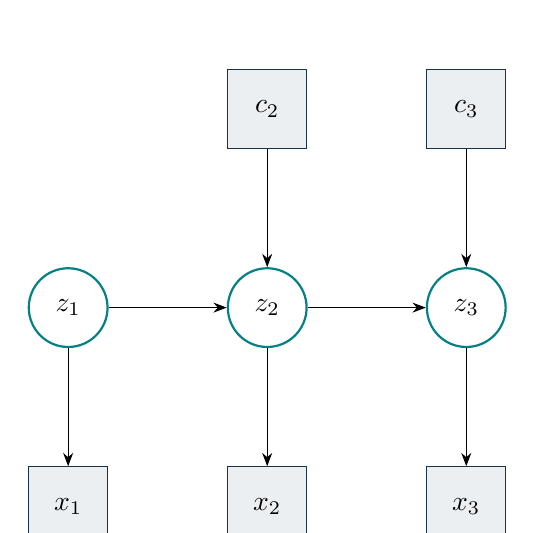
\begin{tikzpicture}[node distance=15mm,>=Stealth, latent/.style={circle,draw=teal,thick,minimum size=10mm},obs/.style={rectangle,draw=navy,minimum size=10mm,fill=navy!8}]
\node[latent](z1){$z_1$};\node[latent,right=of z1](z2){$z_2$};\node[latent,right=of z2](z3){$z_3$};
\node[obs,below=of z1](x1){$x_1$};\node[obs,below=of z2](x2){$x_2$};\node[obs,below=of z3](x3){$x_3$};
\node[obs,above=of z2](c2){$c_2$};\node[obs,above=of z3](c3){$c_3$};
\draw[->](z1)--(z2);\draw[->](z2)--(z3);\draw[->](z1)--(x1);\draw[->](z2)--(x2);\draw[->](z3)--(x3);\draw[->](c2)--(z2);\draw[->](c3)--(z3);
\end{tikzpicture}
\end{center}
\[
p(z,x,m\mid c,\theta)=\pi_{z_1}w_{z_1m_1}p(x_1\mid z_1,m_1)
\prod_{t=2}^T A_{z_{t-1}z_t}(c_t)w_{z_tm_t}p(x_t\mid z_t,m_t).
\]
Conditional independence of observations given latent states and components permits dynamic programming. The first-order Markov assumption is testable through posterior predictive checks; it is not a claim about the LLM architecture.

\textbf{Bayes theorem.} For parameters $\theta$ and all training trajectories $D$,
\[
p(\theta,z,m\mid D)\propto p(\theta)p(z,m,D\mid\theta).
\]
The evidence $p(D)=\int\sum_{z,m}p(D,z,m\mid\theta)p(\theta)d\theta$ normalizes the posterior. The conventional EM model estimates a point $\hat\theta$; the fully Bayesian model integrates parameter uncertainty. Distinguish conditional state posterior from parameter posterior.

\textbf{Emission likelihood.}
\[
b_j(x)=\sum_{m=1}^2 w_{jm}\prod_{d=1}^3\frac{\exp[-(x_d-\mu_{jmd})^2/(2v_{jmd})]}{\sqrt{2\pi v_{jmd}}}.
\]
Fit feature standardization on training data only; handle constant columns explicitly. Store scale, feature order and floating-point precision. Compute log densities and log-sum-exp to prevent underflow. Mixtures express multimodality but introduce component label switching; state identity requires validation.

\sectionpage{Exact sequential inference}
\textbf{Causal filtering.} $f_t(j)=p(z_t=j\mid x_{1:t},c_{1:t},\theta)$.
Prediction $q_t(j)=\sum_i f_{t-1}(i)A_{ij}(c_t)$; for $t=1$, $q_1=\pi$.
\[
f_t(j)=\frac{b_j(x_t)q_t(j)}{\sum_k b_k(x_t)q_t(k)}.
\]
Example: $q_t=(.75,.20,.05)$ and relative densities $(1,2,8)$ give $f_t(H)=.40/1.55=.258$. A persistent prior can delay detection of abrupt changes.

\textbf{Forward recursion.} $a_1(j)=\pi_j b_j(x_1)$ and
$a_t(j)=b_j(x_t)\sum_i a_{t-1}(i)A_{ij}(c_t)$.
The likelihood is $L=\sum_j a_T(j)$. In log space replace sums by log-sum-exp; scaling constants are another valid implementation.

\textbf{Backward recursion.} $r_T(j)=1$ and
$r_t(i)=\sum_jA_{ij}(c_{t+1})b_j(x_{t+1})r_{t+1}(j)$.
Smooth with $\gamma_t(j)=a_t(j)r_t(j)/L$ and
\[
\xi_t(i,j)=\frac{a_t(i)A_{ij}(c_{t+1})b_j(x_{t+1})r_{t+1}(j)}{L}.
\]
$\gamma$ and $\xi$ are posterior sufficient statistics for training, not live risk. Never display smoothing as an online result.

\textbf{Viterbi.} Compute $\delta_1(j)=\log\pi_j+\log b_j(x_1)$ and
\[
\delta_t(j)=\log b_j(x_t)+\max_i[\delta_{t-1}(i)+\log A_{ij}(c_t)].
\]
Record maximizing predecessor, backtrack from terminal maximum. Resolve ties by lowest index. Viterbi is the jointly most probable path, not marginal per-turn argmax.

\textbf{Complexity.} Per turn $O(K^2+KMd)$; forward--backward costs $O(T(K^2+KMd))$ with $O(TK)$ state-message memory. Reset at dossier boundaries. Test exact enumeration of $3^5$ paths, likelihood, marginals, $\xi$, Viterbi and prefix invariance. For one turn, no transition count exists.

\sectionpage{Maximum likelihood and state identity}
Use Baum--Welch as the transparent point-estimation comparator. The complete log likelihood is a sum of initial-state, transition, mixture-weight and Gaussian terms. At EM iteration $r$, evaluate conditional responsibilities under current parameters:
\[
\rho_{ntjm}=\gamma_{nt}(j)\frac{w_{jm}\mathcal N(x_{nt};\mu_{jm},V_{jm})}{b_j(x_{nt})}.
\]
Update $\pi_j=N^{-1}\sum_n\gamma_{n1}(j)$ and
$A_{ij}=\sum_{nt}\xi_{nt}(i,j)/\sum_{ntk}\xi_{nt}(i,k)$.
\par Then $w_{jm}=\sum_{nt}\rho_{ntjm}/\sum_{ntm'}\rho_{ntjm'}$,
\[
\mu_{jm}=\frac{\sum_{nt}\rho_{ntjm}x_{nt}}{\sum_{nt}\rho_{ntjm}},
\quad
v_{jmd}=\frac{\sum_{nt}\rho_{ntjm}(x_{ntd}-\mu_{jmd})^2}{\sum_{nt}\rho_{ntjm}}.
\]
Use three seeded starts, variance floor, empty-component policy and iteration cap. Log likelihood by iteration, occupancy, convergence and meaningful drops; floors can alter strict EM monotonicity. Select highest training likelihood, not test AUROC.

\textbf{Identifiability.} The likelihood is unchanged by simultaneous permutation of latent state indices, and mixture components may switch inside each state. Map the three states to G/U/H using all six permutations on validation labels, maximizing class-balanced posterior agreement. Freeze mapping and report confusion/occupancies. If a class is absent or mapping unstable, report ambiguity rather than asserting semantic regimes. For Bayesian draws align states to a fixed training-derived reference using deterministic assignment; map the reference using validation only; report ambiguous alignments, and use permutation-invariant predictive checks.

\textbf{Matched static baseline.} Let $\bar\pi_j$ be mean training occupancy. Static scores \[s_j(x)=\bar\pi_jb_j(x)/\sum_k\bar\pi_kb_k(x)\] use the identical trained emissions, scaler and mapping. A negative control sets every row of $A$ and initial $\pi$ to $\bar\pi$; its causal scores must equal static scores. This isolates information contributed by transition history rather than features or capacity.

\sectionpage{Fully Bayesian HMM: priors and posterior}
Use conjugate priors for a homogeneous HMM with diagonal Gaussian mixtures. Standardized features support weakly informative priors; prior scales below are initial protocol choices subject to prior predictive checks, not tuned on test.
\[
\pi\sim\mathrm{Dirichlet}(1,1,1),\quad
A_{i:}\sim\mathrm{Dirichlet}(\alpha_{i1},\alpha_{i2},\alpha_{i3}),
\quad w_j\sim\mathrm{Dirichlet}(1,1).
\]
Set $\alpha_{ij}=1+\kappa\mathbf 1(i=j)$ with default $\kappa=0$; compare sticky $\kappa=2,5$ as sensitivity. A strong sticky prior can manufacture apparent persistence.
\[
v_{jmd}\sim\mathrm{InvGamma}(a_0,b_0),\qquad
\mu_{jmd}\mid v_{jmd}\sim N(m_0,v_{jmd}/k_0).
\]
Use $a_0=3,b_0=2,m_0=0,k_0=.5$. Inverse gamma uses density proportional to $v^{-a-1}\exp(-b/v)$. Prior predictive simulate feature scales and dwell times before fitting.

\textbf{Conjugacy.} Given sampled paths, let $N_{ij}$ count transitions, $N_j^{(0)}$ initial states and $N_{jm}$ component assignments. Then
\[
A_{i:}\mid z\sim\mathrm{Dirichlet}(\alpha_{i:}+N_{i:}),\qquad
\pi\mid z\sim\mathrm{Dirichlet}(1+N^{(0)}),
\]
and $w_j\mid m,z\sim\mathrm{Dirichlet}(1+N_{j1},1+N_{j2})$.
For one component and feature containing $n$ assigned observations, mean $\bar x$, and sum of squared deviations $S$:
\[
k_n=k_0+n,\quad m_n=(k_0m_0+n\bar x)/k_n,\quad a_n=a_0+n/2,
\]
\[
b_n=b_0+S/2+\frac{k_0n(\bar x-m_0)^2}{2k_n}.
\]
Draw $v\sim\mathrm{InvGamma}(a_n,b_n)$ and $\mu\sim N(m_n,v/k_n)$. For empty components draw from the prior. The posterior mean transition is $(\alpha_{ij}+N_{ij})/\sum_k(\alpha_{ik}+N_{ik})$; a credible interval is obtained from draws.

\sectionpage{Gibbs, FFBS, MH and HMC/NUTS}
\textbf{Gibbs sampler.} Alternate (i) sample each trajectory $z$ using forward-filtering backward-sampling (FFBS), (ii) sample mixture component $m_t$ proportional to $w_{z_tm}\mathcal N(x_t;\mu,V)$, (iii) update parameters with conjugate conditional draws. FFBS samples $z_T\sim f_T$ and then
\[
p(z_t=i\mid z_{t+1}=j,x_{1:T},\theta)\propto f_t(i)A_{ij}(c_{t+1}).
\]
Sequential dependence is handled by sampling entire paths, not isolated state updates. Use independent chains, seeded initialization, burn-in/warmup, and saved posterior draws. Do not average unaligned states.

\textbf{Metropolis--Hastings.} For nonconjugate parameters $\beta$, a proposal $q(\beta'\mid\beta)$ is accepted with probability
\[
\min\left(1,\frac{p(D\mid\beta')p(\beta')q(\beta\mid\beta')}{p(D\mid\beta)p(\beta)q(\beta'\mid\beta)}\right).
\]
Implement as a small-model educational comparator; tune proposal during warmup only and report acceptance, autocorrelation and mixing. Random-walk MH is not the preferred high-dimensional solution.

\textbf{HMC/NUTS.} Marginalize discrete paths and mixture indicators via differentiable log-forward recursion. For continuous parameter vector $\theta$, potential $U=-\log p(\theta\mid D)$, momentum $r\sim N(0,M)$, Hamiltonian $\mathcal H=U+\frac12r^TM^{-1}r$. Leapfrog updates approximate motion; Metropolis correction restores target invariance. NUTS adapts path length and step size, avoiding manual trajectory choice. Transform simplex/positive parameters with correct Jacobians through PyMC or equivalent. NUTS must not directly sample discrete $z$.

\textbf{Diagnostics.} Start four chains (e.g. 1000 tuning and 1000 retained draws per chain, adjust based on diagnostics). Report rank-normalized split $\widehat R$ (target $\le1.01$), bulk/tail ESS (target at least 400 for key contrasts), Monte Carlo SE, traces and autocorrelation. For NUTS report divergences, tree-depth saturation and energy/BFMI. Diagnose failures; increase draws, reparameterize, simplify or report unavailable. Do not interpret unstable coefficients.

\sectionpage{Covariate-dependent transitions and hierarchy}
Standard HMM assumes time-homogeneity. Use pre-answer standardized covariates $c_{nt}\in\R^p$ in an input-dependent HMM:
\[
A_{ij}(c)=\frac{\exp(\alpha_{ij}+\beta_{ij}^Tc)}{\sum_{k=1}^3\exp(\alpha_{ik}+\beta_{ik}^Tc)}.
\]
Fix destination 3 logits to zero for each origin: $\alpha_{i3}=0,\beta_{i3}=0$. This resolves additive softmax redundancy (not latent-label switching). Use $\alpha_{ij}\sim N(0,1.5^2)$ and $\beta_{ij,k}\sim N(0,\sigma_k^2)$, $\sigma_k\sim\mathrm{HalfNormal}(.5)$, in standardized units. The shared scale shrinks poorly supported effects; compare fixed weakly informative scales via sensitivity. Start with a small preregistered subset (evidence, ambiguity, distractor load, turn number); correlated factors may make effects inseparable. Do not use all possible covariates indiscriminately.

\textbf{Partial pooling.} If enough groups exist, add question-type or domain variation $u_{g,ij}\sim N(0,\tau_{ij}^2)$ with half-normal scale and noncentered $u=\tau\eta$, $\eta\sim N(0,1)$. A single model cannot identify between-model variation; do not fit a model-family hierarchy until multiple checkpoints exist. Dossier random effects are a sensitivity model: integrate new-dossier effects over their population prior at test time, never estimate from test labels.

\textbf{Inference.} Optimize marginal likelihood for a small deterministic initialization, then sample continuous parameters using NUTS with the hidden paths marginalized. For auditing, reconstruct conditional paths with FFBS for posterior draws. If the full mixture transition model is computationally unstable, first fit a single-Gaussian covariate HMM; explicitly distinguish it from the matched two-component primary model.

\textbf{Advanced extension.} A hidden semi-Markov model replaces geometric state dwell times with explicit duration distribution $D_j$, e.g. shifted negative binomial $D_j=1+\mathrm{NB}(r_j,p_j)$. Use segment dynamic programming with a duration cap and correct right censoring at sequence end. Six-turn sequences give weak duration identification: defer this extension unless longer synthetic or real trajectories support it.

\sectionpage{Factor attribution and counterfactual estimands}
For a fixed origin state $i$, factor $c_k$, compare a meaningful low and high value while holding other observed covariates constant. For posterior draw $s$,
\[
\Delta^{(s)}_{i,k}(c)=A^{(s)}_{iH}(c_{k}=h)-A^{(s)}_{iH}(c_k=l).
\]
Average over eligible observed covariate profiles to obtain a standardized risk difference. Report posterior median, 95\% credible interval and $\Prob(\Delta_{i,k}>0\mid D)$. Avoid extrapolation outside common support. A logit coefficient relative to the reference destination is not itself a risk difference; softmax competition changes all probabilities.

\textbf{Filter-weighted contrast.} Given previous state distribution $f_{t-1}$, effect on entering H before observing the next answer is
\[
\Delta_k=\sum_i f_{t-1}(i)[A_{iH}(c_k=h)-A_{iH}(c_k=l)].
\]
Separate entering H from remaining H; report effects by origin and sample contribution. For post-answer feature attribution, remove one feature by analytically marginalizing that coordinate from each diagonal Gaussian component. Compute $f_t(H)-f_t^{(-d)}(H)$, holding prior and other observed coordinates fixed. Effects are order-independent leave-one-out contrasts, not additive decompositions or causal effects. Optionally calculate Shapley values across the eight subsets of the three features to allocate the total posterior risk difference; define the empty subset as the predictive prior. 

\textbf{Controlled intervention.} At a preregistered eligible prefix, randomize paired branches to original previous answer vs verified correction. Keep subsequent question, generation settings and evidence constant; use matched seeds where possible, independent replication across dossiers, and avoid treating multiple branches as independent. A separate factorial design manipulates evidence restoration and distractor context. Grade next-turn unsupported error independently. The primary estimand is an intention-to-treat risk difference $\E[Y(1)-Y(0)]$ in the eligible population, where $Y=1$ indicates next-turn H. Report paired counts and uncertainty. A Bayesian paired logistic model with dossier intercept may estimate standardized differences; bootstrap pairs as a robustness check. Selection on already wrong prefixes restricts generalization. No counterfactual claim from observational $A(c)$ alone.

\sectionpage{Forecasting and Bayesian decision theory}
\textbf{Next-turn risk.} Current answer detection uses $f_t$; prospective risk without seeing the next answer is
\[
r_{t+1}=\E_{\theta\mid D,x_{1:t}}[f_t^{\theta} A^\theta(c_{t+1})]_H.
\]
For an unknown future covariate, integrate over a stated scenario distribution rather than pretend it is observed. In fixed-parameter homogeneous inference $f_{t+h}=f_t A^h$; this is state occupancy at horizon $h$, not probability of any error by $h$. Compute first-entry probability using submatrix $Q=A_{\neg H,\neg H}$: conditional on the current non-H state distribution $g_t$, $1-g_t Q^h\mathbf 1$. For changing covariates, use ordered products of $Q(c)$. If current truth is unknown, clearly distinguish model posterior currently non-H from known audit labels.

\textbf{Posterior integration.} For posterior draws from training, use equal-weight approximation when explicitly treating parameters as frozen for deployment. For exact Bayesian prediction conditional on a new observed prefix, reweight draws by their prefix likelihood $p(x_{1:t}\mid\theta_s)$; normalize with log-sum-exp and monitor importance ESS. Compare plug-in, frozen ensemble and reweighted predictions; if weights collapse report limitation or use sequential Monte Carlo resampling/rejuvenation. Posterior risk mean and quantiles describe uncertainty in latent-state probability, not a confidence interval for a realized binary outcome.

\textbf{Bayesian decision theory.} For alert cost $C_{FP}$ on non-H and missed-error cost $C_{FN}$ when H, alert if
$r>C_{FP}/(C_{FP}+C_{FN})$ under a one-step loss model. A multi-turn stop changes future opportunities, so use a separate empirical first-alarm policy or optional dynamic programming under explicit action-dependent costs. Select validation thresholds under a maximum 5\% false-stop rate on clean conversations, handling ties and never-alert. Do not claim a stop prevents the already-generated hallucination. Guarded output is excluded from uninterrupted evaluation.

\sectionpage{Simulation, calibration and statistical validation}
Simulation is mandatory before expensive collection. Include (1) independent states (identical $A$ rows), (2) persistent states, (3) abrupt onset, (4) overlapping G/U/H emissions, (5) high-confidence wrong answers and (6) covariate effects with known coefficient signs, including null and confounded scenarios. Generate known priors and recover parameters up to permutations. Run repeated seeded datasets of different sizes. Report bias, RMSE, interval coverage, false discoveries, calibration and compute time. Simulation-based calibration: sample parameters from prior, simulate data, fit posterior, check rank uniformity for permutation-invariant or consistently identified quantities. Use enough replications to distinguish Monte Carlo noise from defects.

\textbf{Primary endpoint.} Define $\tau_n=\min\{t:y_{nt}=H\}$; no H means $\tau=\infty$. In the onset risk set keep $t\le\tau$ and label $1$ only at $\tau$. For G,U,H,H,G retain targets 0,0,1. Unresolved earlier labels make onset ambiguous; report excluded dossiers. All-turn state detection is secondary. Next-turn prediction at $t$ targets $y_{t+1}=H$ and uses only information available through $t$ plus known next-question conditions.


\begin{tabularx}{\linewidth}{p{.27\linewidth}X}
\toprule Metric & Definition or purpose \\ \midrule
AUROC / average precision & Ranking quality; AP interpreted with onset prevalence. Undefined AUROC for single class. \\
Brier score & $N^{-1}\sum_i(p_i-y_i)^2$; probabilistic accuracy. \\
Log score & $-N^{-1}\sum_i[y_i\log p_i+(1-y_i)\log(1-p_i)]$; proper scoring. \\
Calibration & Reliability curve, calibration intercept/slope, bin counts; ECE exploratory and bin-sensitive. \\
Alarm outcomes & Clean false stop, premature, on-time, delayed, miss, clean no-alarm; delay only among on-time/delayed. \\
Uncertainty & At least 500 paired whole-dossier bootstrap replicates, preferably 2000; report valid count and percentile 95\% intervals. \\ \bottomrule
\end{tabularx}

\textbf{Model comparison.} M0 single feature selected on validation; M1 matched static mixture; M2 EM-HMM; M3 Bayesian homogeneous HMM; M4 Bayesian covariate HMM. Compare on the same feature set, same eligibility, held-out IDs and frozen label mapping. Bayesian posterior predictive checks compare simulated vs observed feature ranges, error durations (only where semantics validated), transition counts and distribution of onset times. For WAIC/PSIS-LOO use full dossier marginal likelihood as pointwise unit; check Pareto-$k$ and use grouped cross-validation when unreliable. Do not report Bayes factors without proper priors and stable marginal likelihood. Hold-out performance remains primary.

\sectionpage{Visual analytics and research dashboard}
Dashboard is read-only over saved artifacts; it must never refit models or alter the locked test set. Every view displays run ID, synthetic/real status, data split, model and eligibility count.

\begin{tabularx}{\linewidth}{p{.28\linewidth}X}
\toprule View & Required contents \\ \midrule
Trajectory explorer & Three stacked state posterior curves or probability ribbons; reference labels shown separately; first error, alarm and next-turn forecast. Toggle causal filter vs retrospective smoother with obvious distinction. \\
Transition heatmap & Rows origin, columns destination; posterior mean and credible interval; dynamic covariate scenario selector; compare empirical label transitions. \\
Factor forest plot & Risk-difference estimates and 95\% credible intervals around zero; probability of positive effect, origin state and sample count. \\
Evidence gap audit & Visible evidence, question and generated answer; feature contributions; independent grade and explanation categories. \\
Posterior diagnostics & Trace, rank, ESS, $\widehat R$, autocorrelation and divergence summary; warning for unstable inference. \\
Performance & ROC/PR, calibration, score comparison, paired bootstrap differences and first-alarm counts. \\
Forecast & Probabilities by horizon and parameter credible bands; occupancy vs first-entry probability. \\
Intervention & Branch-level paired outcomes, risk difference and uncertainty; separate control/intervention dataset. \\ \bottomrule
\end{tabularx}

\begin{center}
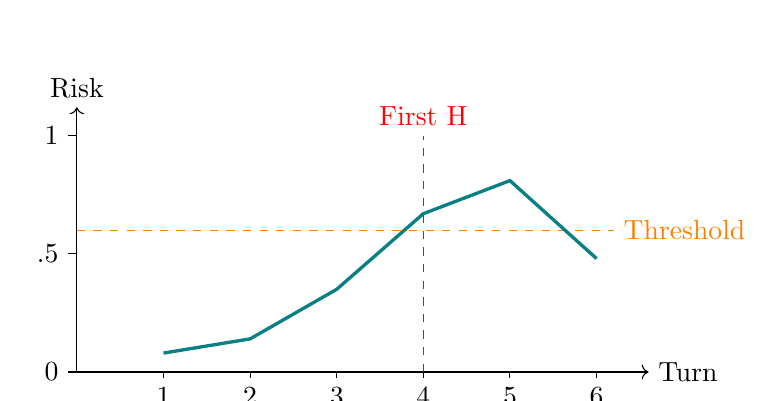
\begin{tikzpicture}[x=1.1cm,y=3cm]
\draw[->] (0,0)--(6.6,0) node[right]{Turn};
\draw[->] (0,0)--(0,1.12) node[above]{Risk};
\foreach \x in {1,...,6}{\draw(\x,0)--(\x,-.025)node[below]{\x};}
\foreach \y in {0,.5,1}{\draw(0,\y)--(-.1,\y)node[left]{\y};}
\draw[dashed,orange] (0,.6)--(6.2,.6)node[right]{Threshold};
\draw[dashed,red] (4,0)--(4,1);
\draw[very thick,teal] plot coordinates{(1,.08)(2,.14)(3,.35)(4,.67)(5,.81)(6,.48)};
\node[red,anchor=south] at (4,1){First H};
\end{tikzpicture}
\end{center}
\small Illustrative design only: a high posterior at turn 4 is not a measured result. In the implemented chart, uncertainty bands are drawn from posterior samples and all alerts come from frozen validation thresholds.

\sectionpage{Software architecture and data contracts}

\begin{tabularx}{\linewidth}{p{.36\linewidth}X}
\toprule Module & Responsibility \\ \midrule
config/ & Typed run config, versioned schemas, seed derivation, manifest fingerprint. \\
data/dossiers.py & Seeded generation, split ownership, fixtures, JSON validation. \\
data/collector.py & Optional MLX adapter, atomic recording, resume, timing and failure ledger. \\
data/grader.py & Deterministic grading and blinded review queue, separate label store. \\
features/ & Causal feature extraction, training-only scaler, missingness protocol. \\
models/emissions.py & Diagonal mixture densities, stable log-sum-exp. \\
models/hmm.py & Filtering, smoothing, Viterbi, Baum--Welch, static control. \\
models/bayes.py & Dirichlet/NIG updates, FFBS Gibbs, posterior draw storage. \\
models/covariate.py & Softmax transitions, marginalized likelihood, NUTS. \\
inference/ & Forecast, feature and transition contrasts, decision policy. \\
evaluation/ & Frozen splits, metrics, paired bootstrap, intervention estimands. \\
reporting/ and dashboard/ & Read-only report generation, plots, Streamlit/Plotly interface. \\
tests/ & Numerical oracles, data contracts, diagnostics, integration, leakage tests. \\ \bottomrule
\end{tabularx}

\textbf{Interfaces.} Detector receives only ordered finite feature vector, available covariates and previous posterior. Provide \texttt{step(x, previous=None)}, \texttt{filter(sequence)}, \texttt{smooth(sequence)}, \texttt{viterbi(sequence)}, \texttt{fit(train)}, \texttt{save/load}, \texttt{forecast(state, horizon, scenario)}. Grading record must not cross the detector boundary. Keep raw immutable JSON per dossier, separate grade files, split manifest and model/scaler bundle. Export posterior draws NetCDF or NPZ; save predictions and evaluation as CSV/JSON with schema version.

\textbf{Artifacts.} \texttt{manifest.json}, \texttt{splits.json}, \texttt{report.json}, \texttt{test\_audit.csv}, \texttt{model.npz}, \texttt{posterior.nc}, \texttt{guard.npz}, \texttt{figures/}, \texttt{results.md}. No fake Qwen outputs. A missing hardware stage remains explicitly pending. Keep core imports independent of MLX, PyMC and dashboard optional extras.

\sectionpage{Implementation milestones and acceptance criteria}
\begin{enumerate}
\item \textbf{M0 Baseline inspection.} Extract starter if available, preserve example outputs, run existing verify and demo. Record actual code and dependencies; use compatible clean implementation if unavailable.
\item \textbf{M1 Contracts and fixtures.} Deterministic dossiers, grading, split ownership, manifest, mocked generator and atomic resume. Test wrong-entity codes, shared codes, legitimate abstentions, malformed and empty outputs.
\item \textbf{M2 Exact HMM.} Forward/backward, filtering, mixture EM, Viterbi, negative control. Compare every quantity with enumeration; row sums and save/load parity within $10^{-8}$ in float64; prefix invariance; no cross-boundary transitions.
\item \textbf{M3 Bayesian core.} Conjugate Gibbs/FFBS, prior checks, synthetic recovery, chain diagnostics, state mapping. Derive each update in accompanying notebook; verify against conjugate toy cases.
\item \textbf{M4 Attribution.} Covariate softmax, marginalized likelihood checked against brute force, NUTS on synthetic null/non-null scenarios, posterior contrasts and feature removal. Validate no future information.
\item \textbf{M5 Pilot.} Run five MLX dossiers on Apple silicon; inspect probability extraction, token termination, grades, timing, memory, feature ranges and clean/affected counts. Freeze settings; estimate full runtime as seconds/dossier times 500.
\item \textbf{M6 Locked collection.} Generate 500 dossiers sequentially within each trajectory; resume compatible records; blind review labels. Do not change prompt or feature definition after test access.
\item \textbf{M7 Evaluation.} Fit train only, choose mapping/hyperparameters/threshold on validation, open test once; paired bootstrap, all-turn/onset/forecast and alarm results.
\item \textbf{M8 Intervention and reporting.} Separate randomized branch experiment; produce figures, dashboard and paper-style report. Complete integrity checks and record commands and limitations.
\end{enumerate}

\textbf{Release gates.} All core unit and integration tests pass offline. Exact oracle and leakage tests pass. Synthetic experiments labeled synthetic. Real metrics exist only after valid real collection. Unresolved mapping, diagnostics or sparse onset rates explicitly constrain claims. Report any unexecuted stage, rather than invent results.

\sectionpage{Execution plan and commands}
The implementing agent may edit, run and test files directly on the Mac; an additional IDE is optional. Use an isolated project directory, Python environment and Git history. Python 3.11/3.12 is preferred for scientific stack compatibility; verify the installed package versions and Apple silicon runtime before pinning them. No dependence on a paid API for the core study.

The following are intended interface contracts, not commands verified against an implemented project yet:
\begin{verbatim}
python -m venv .venv
source .venv/bin/activate
python -m pip install -e '.[dev,bayes,ui]'
python verify.py
python evaluate.py --demo --out simulation
python -m pip install -e '.[mlx]'
python collect.py --start 10000 --count 5 --dir pilot
python collect.py --count 500 --dir rollouts
python evaluate.py --dir rollouts --out results
python -m regime_lab.bayes --dir rollouts --out results/bayes
python -m regime_lab.report --results results
streamlit run dashboard/app.py
python collect.py --start 20000 --count 5 --dir live \
    --guard results/guard.npz
\end{verbatim}
Use an actual locked dependency file after successful installation; retain baseline CLI compatibility. Use offline fixtures when network or weights are unavailable. Dashboard access may be via local browser while code and terminal remain in the development environment. Keep UI separate from scientific logic.

\textbf{Resource planning.} CPU NumPy EM and synthetic work are first; actual MLX model generation dominates collection; NUTS performance depends on sequence count, mixture size and computational graph. Profile a small covariate model first, then increase sample sizes. Save checkpoints and draw diagnostics; do not promise a full MCMC run duration before benchmarking.

\textbf{Build instruction.} Upon approval, follow milestones M0--M8, preserve the existing project, run all authorized offline stages, fix recoverable failures, and stop only for true dependencies that require user action. Return the actual implementation, verification results and limitations, not another plan.

\sectionpage{Research integrity, deliverables and references}
\textbf{Threats to validity.} A fictional short-code task may not generalize to natural-language hallucinations; lexical similarity may confuse wrong entities; entropy reflects output difficulty, not truth; state persistence can reflect conversation or dossier difficulty; short sequences limit duration inference; repeated branch outcomes are dependent; annotation gaps may alter onset coverage; label switching limits semantic interpretations. Mitigate with independent grading, group splits, matched emissions, prior sensitivity, transparent coverage, paired controls and reporting of null findings. External validity to other checkpoints and domains is future work.

\textbf{Submission package.} Research paper-style report (abstract, problem, related work, model derivations, experimental design, results, uncertainty and limitations); reproducible CLI package; independent raw/label data and manifests; notebooks explaining Bayes/FFBS and simulation checks; figures and interactive dashboard; reproducibility and test report; concise presentation and oral defense based on actual results.

\textbf{Course defense.} Explain why HMM filtering differs from smoothing, why EM is not full Bayesian inference, why Dirichlet/NIG conjugacy works, how FFBS samples dependent paths, why NUTS marginalizes discrete states, why priors and label switching matter, how credible intervals differ from bootstrap intervals, and why a covariate effect is not necessarily causal.

\textbf{Reference starting points.} The attached research report supplies the project-specific literature survey and reported simulation findings. The following established methods and papers are recommended reading; verify bibliographic details and links during the build before using them in a formal paper.
\begin{enumerate}[leftmargin=*]
\item Rabiner, L. R. (1989). A tutorial on hidden Markov models and selected applications in speech recognition. \emph{Proceedings of the IEEE}.
\item Gelman et al. \emph{Bayesian Data Analysis}, 3rd ed. Chapman and Hall/CRC.
\item Scott, S. L. (2002). Bayesian methods for hidden Markov models: recursive computing in the 21st century. \emph{JASA}.
\item Hoffman and Gelman (2014). The No-U-Turn Sampler. \emph{Journal of Machine Learning Research}.
\item Vehtari et al. (2021). Rank-normalization, folding, and localization: an improved $\widehat R$ for assessing convergence of MCMC. \emph{Bayesian Analysis}.
\item Zhang et al. (2024). How Language Model Hallucinations Can Snowball. ICML.
\item Wu et al. (2024). Synchronous Faithfulness Monitoring for Trustworthy Retrieval-Augmented Generation. EMNLP.
\item Niu et al. (2024). RAGTruth: A Hallucination Corpus for Developing Trustworthy Retrieval-Augmented Language Models. ACL.
\item Farquhar et al. (2024). Detecting hallucinations in large language models using semantic entropy. \emph{Nature}.
\end{enumerate}
\textbf{Approval checkpoint.} This document is a blueprint only. No new implementation, real-model experiment, or research claim has been completed.
\end{document}
